\documentclass[11pt]{article}

\usepackage[margin=1in]{geometry}
\usepackage{amsmath,amssymb}
\usepackage{graphicx}
\usepackage{booktabs}
\usepackage{hyperref}
\usepackage{xcolor}
\usepackage{enumitem}
\hypersetup{colorlinks=true,linkcolor=black,citecolor=blue,urlcolor=blue}

\title{\textbf{ProteinTuneRL: A Reinforcement Learning Perspective on\\ Antibody Design}\\[4pt]
\large Algorithms, Correctness Analysis, and Training Behaviour}
\author{Ruman Shaikh}
\date{16 July 2026}

\newcommand{\iglm}{\textsc{IgLM}}

\begin{document}
\maketitle

\begin{abstract}
This report studies \emph{ProteinTuneRL}, a framework that treats antibody
CDR-loop design as constrained reinforcement learning (RL) over amino-acid
tokens. An infilling protein language model (\iglm) provides the policy, and a
cheap structural proxy provides the reward. Alongside the biological framing, the
report makes three technical contributions. First, it adds and formalises an
Advantage Actor-Critic algorithm with Generalized Advantage Estimation (A2C+GAE)
that uses a token-level value function suited to variable-length infills. Second,
it presents a correctness analysis of the online-RL machinery that identifies and
repairs several defects: an incorrectly implemented adaptive KL controller, a
support mismatch between the sampling distribution and the gradient estimate, a
missing bootstrap for truncated episodes in GAE, an action-leaking value baseline
in PPO, and an attention-kernel incompatibility that prevents REINFORCE from
computing gradients. Each repair is covered by a regression test. Third, it
examines a reward-design issue: the default $\beta$-sheet objective is a
compositional amino-acid propensity rather than a structural prediction, and its
signal is diluted when the score is computed over the entire chain. Training runs
of PPO, A2C+GAE, and REINFORCE on a CDR-H3 $\beta$-sheet objective show that all
three improve the reward, that they differ mainly in how far they drift from the
pretrained distribution, and that most useful learning occurs within roughly one
to two thousand steps. The central difficulty in this setting is controlling
divergence from the pretrained biological prior while continuing to improve the
design objective.
\end{abstract}

\section{Introduction}
Proteins are the functional units of biological systems. Their behaviour follows
the principle that sequence determines a folded structure, which in turn
determines function. Recent structure predictors have shown that machine learning
can recover folds at scale, but accurate structure prediction alone does not solve
protein \emph{design}, which also depends on stability, binding behaviour, and
evolutionary constraints.

Antibodies illustrate this difficulty. They bind foreign molecules through short,
flexible \emph{Complementarity Determining Regions} (CDRs), and binding is
sensitive to small changes in sequence. Among the CDRs, CDR-H3 is the most
variable and one of the most influential for binding, which makes it a natural
target for sequence optimisation.

\section{From Antibody Structure to Sequence Modelling}
Antibodies have a characteristic Y-shape whose tips carry the CDR loops
responsible for binding. Although a protein is a sequence, its function depends on
folding, and computing the full three-dimensional fold of every candidate
sequence is too expensive to place inside an optimisation loop. ProteinTuneRL
therefore relies on proxy objectives, meaning cheap signals that correlate with
structural behaviour. One such proxy is $\beta$-sheet propensity, an estimate of
whether a sequence tends to form $\beta$-sheet-like structure. It does not
guarantee correct folding, but it can be evaluated efficiently.

Because a protein can be written as a string over roughly 20 amino acids, it can
be modelled with a language model. ProteinTuneRL is built around
\iglm~\cite{iglm}, an antibody language model designed for \emph{infilling}: a
region such as a CDR loop is masked, and replacements are generated conditioned on
the surrounding context.

\section{Antibody Design as Constrained Reinforcement Learning}
Given a masked target region and a cheap proxy score, antibody infilling can be
posed as a sequential decision problem over discrete symbols:
\begin{itemize}[nosep]
  \item \textbf{State}: the antibody sequence with a masked region and its
  surrounding context.
  \item \textbf{Action}: the choice of amino acid at each masked position.
  \item \textbf{Policy} $\pi_\theta$: the language model's conditional
  distribution over amino acids.
  \item \textbf{Reward}: a scalar proxy (for example, $\beta$-sheet propensity)
  for the completed sequence.
  \item \textbf{Environment}: a deterministic evaluator that scores the
  completion.
\end{itemize}
Supervised learning is insufficient for this task. A model trained on existing
antibodies reproduces the distribution of known sequences, which need not contain
the optimal sequence for a specified objective. Reinforcement learning allows the
policy to depart from imitation, while a \textbf{KL-divergence penalty} toward the
pretrained \iglm~\cite{ziegler} keeps generated sequences within a plausible
region of sequence space. Writing $\pi_{\text{ref}}$ for the frozen reference,
each sampled sequence $y$ receives
\begin{equation}
  r'(y) \;=\; r(y) \;-\; \beta\,\big(\log \pi_\theta(y\mid x) - \log \pi_{\text{ref}}(y\mid x)\big),
  \label{eq:klreward}
\end{equation}
so the objective balances exploration toward higher reward against retention of
the pretrained distribution. The penalty is applied at the reward level and is
therefore common to PPO, A2C, and REINFORCE.

\section{What ProteinTuneRL Does in Practice}
At a high level, ProteinTuneRL lets reinforcement learning operate on protein
sequences without a physics-based simulation inside the training loop. The
workflow is:
\begin{enumerate}[nosep]
  \item start from a real antibody sequence and keep most of it fixed;
  \item mask a small region, usually a CDR loop;
  \item use \iglm{} to fill in the missing amino acids;
  \item score the generated sequence with a proxy objective;
  \item apply reinforcement learning so later generations move toward higher
  scores while remaining close to the pretrained prior.
\end{enumerate}
The system is driven by a single entry point that selects trainers, optimisers,
and evaluators from configuration files. This modular structure makes it a
suitable environment for comparing RL algorithms while the biological setup is
held fixed.

\section{Extensions Implemented}
\subsection{A2C + GAE}
The main algorithmic extension is an Advantage Actor-Critic optimiser with
Generalized Advantage Estimation~\cite{gae}. The motivation is an alternative to
PPO that is lighter to run, more stable than raw REINFORCE, and closer to classical
actor-critic theory. The \iglm{} backbone acts as the actor. A copied backbone
with a scalar linear head acts as the critic and produces a token-level value
$V(s_t)$ for each infill position $t$; a single scalar value is inadequate for
variable-length infills. The terminal reward $r'$ is assigned to the last
generated token, and GAE propagates it backward,
\begin{equation}
  \delta_t = r_t + \gamma\,V(s_{t+1})\,m_{t+1} - V(s_t),
  \qquad
  A_t = \sum_{l\ge 0}(\gamma\lambda)^l\,\delta_{t+l}\,,
  \label{eq:gae}
\end{equation}
where $m_{t+1}$ is a continuation mask, $\gamma=0.99$, and $\lambda=0.95$. The
policy loss is $-\,A_t\,\log\pi_\theta$, the value target is $A_t+V(s_t)$, and an
entropy term is added. Gradient norms of both actor and critic are clipped.

\subsection{REINFORCE as a Baseline}
The framework already includes REINFORCE, which is used here as a baseline. It
applies the raw policy gradient with a mean-reward baseline and an entropy term,
$\nabla_\theta J \approx \mathbb{E}[(r'-\bar r)\,\nabla_\theta\log\pi_\theta(y\mid x)]$.
The baseline makes the optimisation trade-offs of variance and stability easier to
read in a relatively raw form.

\subsection{Explicit KL-Regularised Optimisation}
Maintaining proximity to the pretrained prior is a central concern in protein
design, and the framework supports an explicit KL penalty between the updated
policy and the original \iglm{} (Eq.~\ref{eq:klreward}). Increasing the KL weight
constrains exploration and preserves biological realism; decreasing it allows more
aggressive optimisation of the proxy reward. Because the penalty is applied at the
reward level, it is compatible with PPO, A2C, and REINFORCE.

\section{Correctness Analysis and Fixes}
Extended training of the online algorithms exposed several defects in the shared
machinery. Each was corrected and covered by a unit test (Table~\ref{tab:fixes}).
The corrections apply to all three algorithms where the underlying code is shared.

\begin{table}[h]
\centering
\small
\begin{tabular}{@{}p{3.3cm}p{6.3cm}p{4.3cm}@{}}
\toprule
\textbf{Issue} & \textbf{Defect} & \textbf{Correction} \\
\midrule
Adaptive KL controller &
$\texttt{KL} - \texttt{target}/\texttt{target}$ collapses to $\texttt{KL}-1$ for
any target; the update also made $\beta$ a per-sequence tensor &
Use $(\overline{\mathrm{KL}}-\tau)/\tau$ over the cross-process mean KL, and keep
$\beta$ a scalar synchronised across ranks \\
\addlinespace
On-policy support &
Sampling masks control tokens to $-\infty$, but the gradient recomputed
log-probabilities over the full vocabulary &
Apply the same constrained-support mask when recomputing log-probabilities and
the KL estimate \\
\addlinespace
GAE truncation &
Episodes cut off by \texttt{max\_length} were treated as terminal, so no value
bootstrap was applied &
Record a truncation flag and bootstrap $V(s_T)$ for truncated episodes only \\
\addlinespace
PPO value baseline &
The state-value baseline pooled over the whole sequence, including the generated
action, which biases the gradient &
Condition the value on the prompt tokens only \\
\addlinespace
PPO stability &
No gradient clipping was applied, and the policy could diverge to a non-finite
state under sustained training &
Add gradient-norm clipping and a non-degenerate minibatch for advantage
normalisation \\
\addlinespace
REINFORCE backward &
Under eager attention, an in-place update of the attention mask in the sampling
loop breaks gradient computation &
Use the scaled-dot-product attention implementation for the policy \\
\bottomrule
\end{tabular}
\caption{Defects in the online-RL machinery and their corrections. Pure-tensor
unit tests cover the KL controller, the constraint masking, and the GAE bootstrap;
end-to-end optimiser-step tests cover PPO and A2C.}
\label{tab:fixes}
\end{table}

Two of these defects determine whether an algorithm runs at all. Without gradient
clipping, PPO can train for several thousand steps and then diverge to a
non-finite state; clipping restores a stable trajectory. REINFORCE is incompatible
with the eager attention kernel because it back-propagates through the
autoregressive sampling graph, in which the attention mask is updated in place;
changing the attention implementation removes the in-place operation. The remaining
defects introduce bias rather than failure. The KL-controller and support-mismatch
corrections make the KL regulariser quantitatively meaningful, and the prompt-only
baseline restores an unbiased policy gradient.

\section{Reward Design Considerations}
The default objective is the $\beta$-sheet fraction returned by a standard
biophysics library. This quantity is a compositional statistic. It counts the
fraction of residues whose amino-acid identity belongs to a fixed sheet-favouring
set, and it is not a prediction of secondary structure. Optimising it rewards the
emission of particular residues, which correlates only loosely with the folded
structure and is a weak proxy for a CDR-H3 loop that does not adopt a $\beta$-sheet
conformation.

A second issue is dilution. The score was computed over the concatenated heavy and
light chains, about 230 residues, whereas the policy controls only the roughly 12
infilled CDR-H3 positions. The learnable signal is therefore a small fraction of a
metric dominated by the fixed framework. We add a \texttt{region\_only} option that
scores only the infilled span, which removes the dilution. The normalisation
constants must then be recomputed for the region-only distribution, and its larger
magnitude makes gradient clipping advisable in sensitive optimisers such as PPO.
Structural rewards based on predicted folding remain available at a substantially
higher cost per step.

\section{Results and Training Behaviour}
This section characterises the behaviour of the online algorithms rather than
reporting best-case performance. Each run optimises the CDR-H3 $\beta$-sheet
objective for 2000 steps at batch size 8 under the KL regulariser of
Eq.~\ref{eq:klreward}. Two quantities are tracked: the training reward, which
already includes the negative KL term, and the KL divergence from the pretrained
\iglm{}, which measures policy drift. All curves use a 200-step moving average.

\subsection{PPO}
PPO (Figure~\ref{fig:ppo}) behaves conservatively. The reward rises early and then
settles onto a stable plateau, and the KL increases and then stabilises rather than
growing without bound. Training is smooth, with no large oscillations. This is the
expected behaviour of a clipped update that trades update size for stability in a
high-dimensional discrete action space.

\begin{figure}[h]
\centering
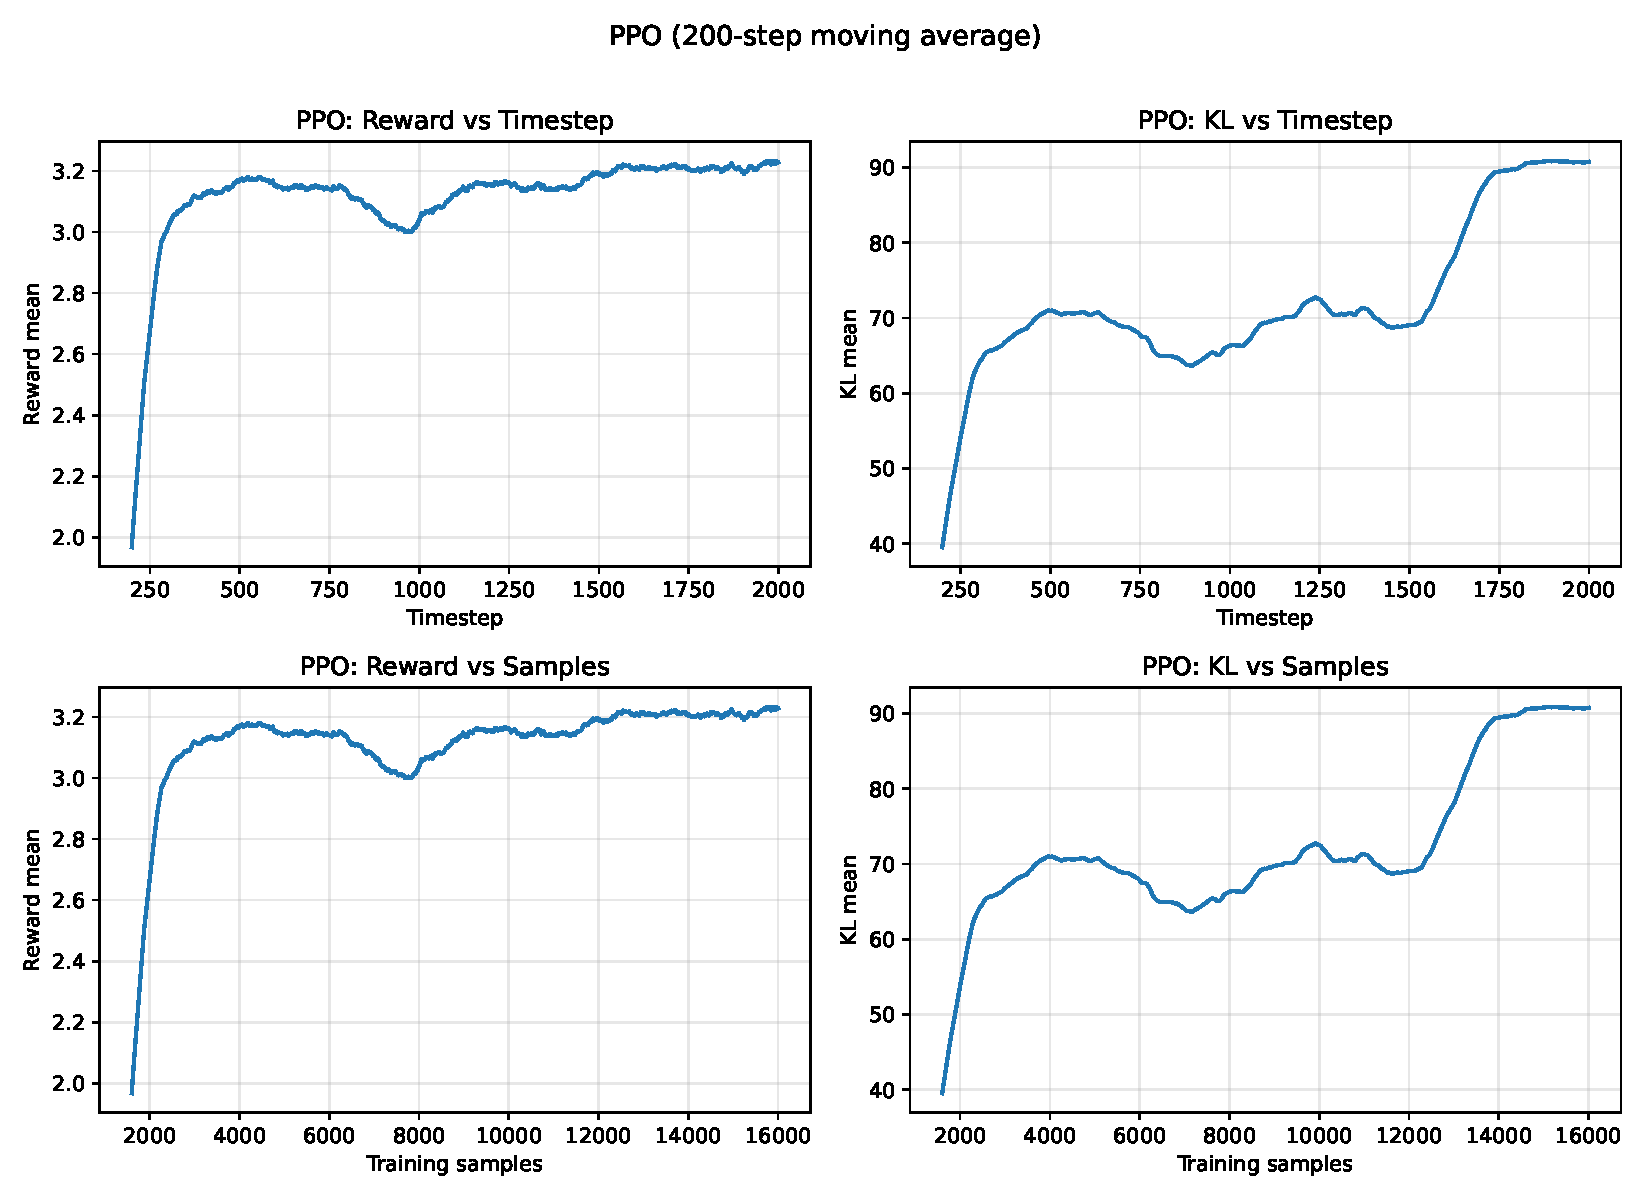
\includegraphics[width=0.9\textwidth]{figures/ppo.pdf}
\caption{PPO: reward and KL divergence against timestep and against training
samples (200-step moving average). Reward plateaus while KL stabilises.}
\label{fig:ppo}
\end{figure}

\subsection{A2C + GAE}
A2C with GAE (Figure~\ref{fig:a2c}) learns with sharper dynamics. The reward climbs
quickly early in training, consistent with the improved credit assignment of the
token-level critic, and the KL grows more aggressively than for PPO. In these runs
A2C reaches a comparable reward at roughly half the final KL divergence of PPO and
REINFORCE, which indicates that the advantage estimate concentrates updates where
they are informative. Without PPO-style clipping the policy retains more freedom to
drift later in training, which is the reason gradient clipping is applied to the
actor and critic.

\begin{figure}[h]
\centering
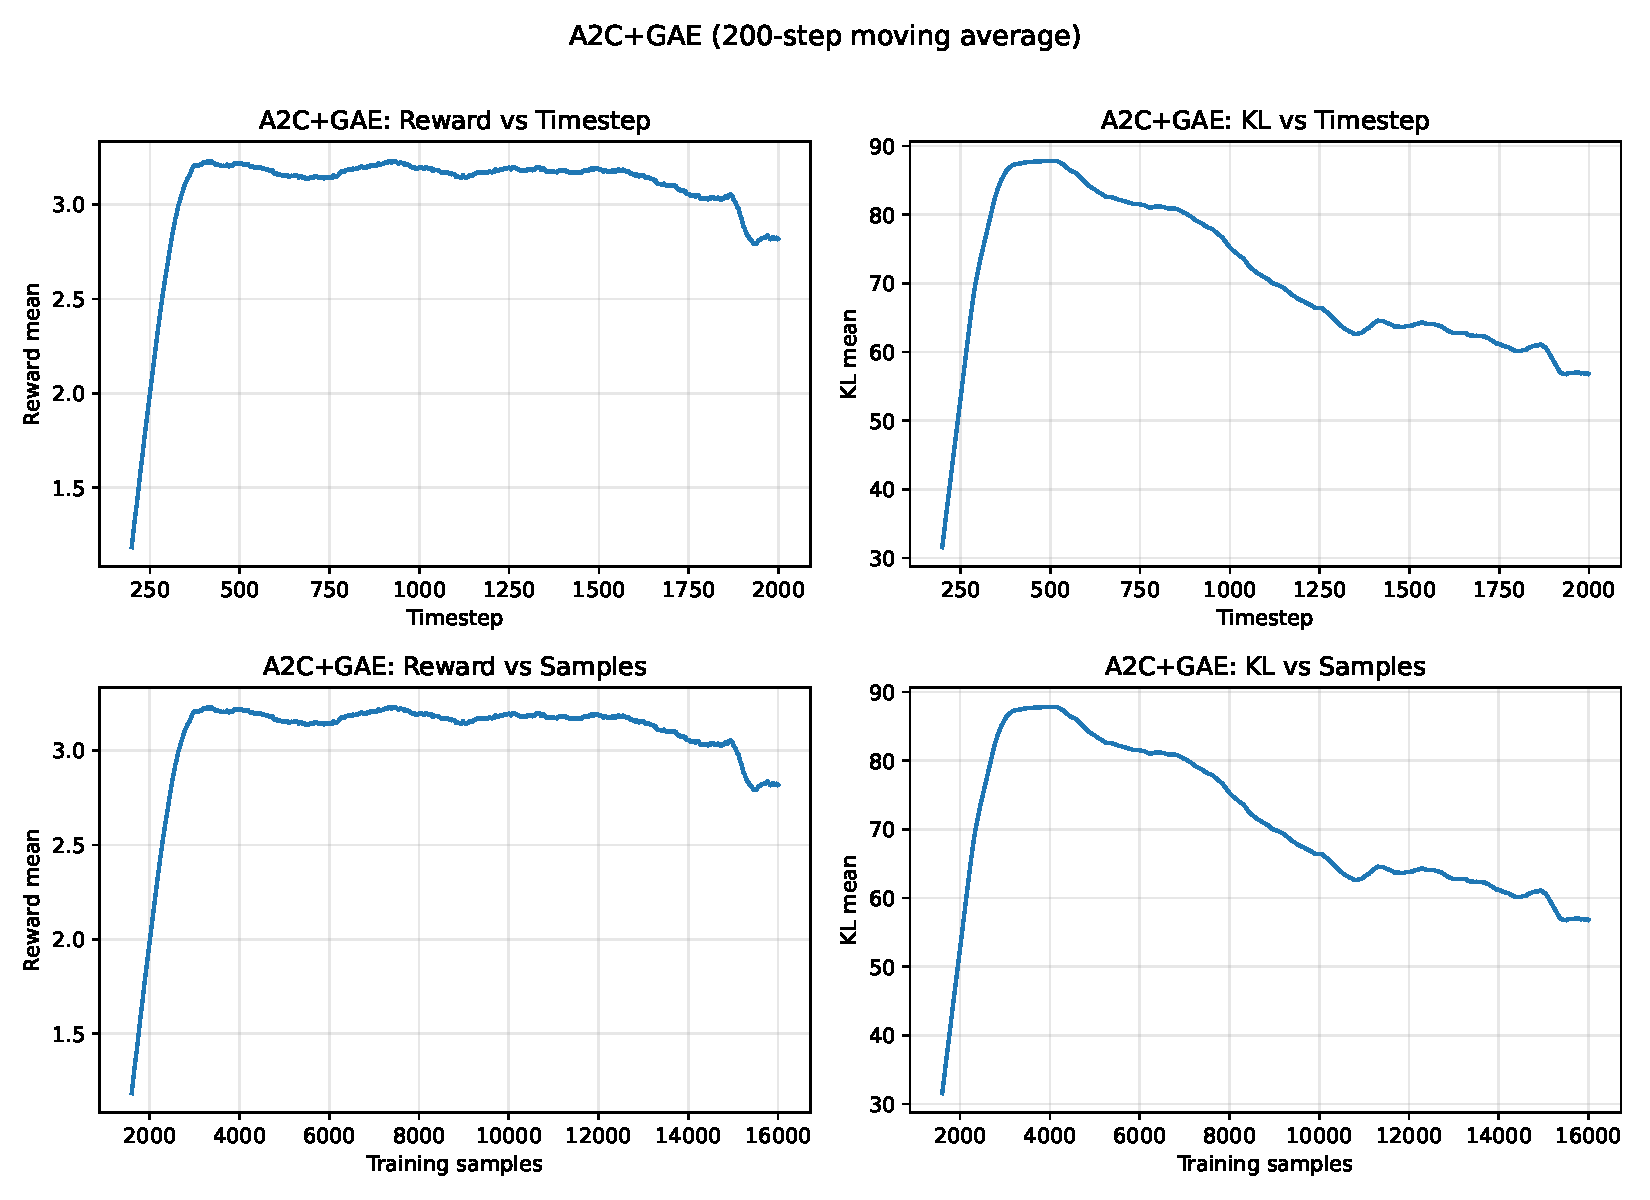
\includegraphics[width=0.9\textwidth]{figures/a2c.pdf}
\caption{A2C+GAE: faster early reward gains and a lower final KL than PPO and
REINFORCE in these runs, with a greater tendency to drift late in training.}
\label{fig:a2c}
\end{figure}

\subsection{REINFORCE}
REINFORCE (Figure~\ref{fig:reinforce}) behaves as a high-variance policy-gradient
baseline. The reward improves but noisily, the KL grows steadily with limited
self-correction, and convergence is slower and less reliable than for PPO or A2C.
This baseline confirms that the optimisation signal is present and shows why
variance reduction and trust-region constraints are useful in sequence design.

\begin{figure}[h]
\centering
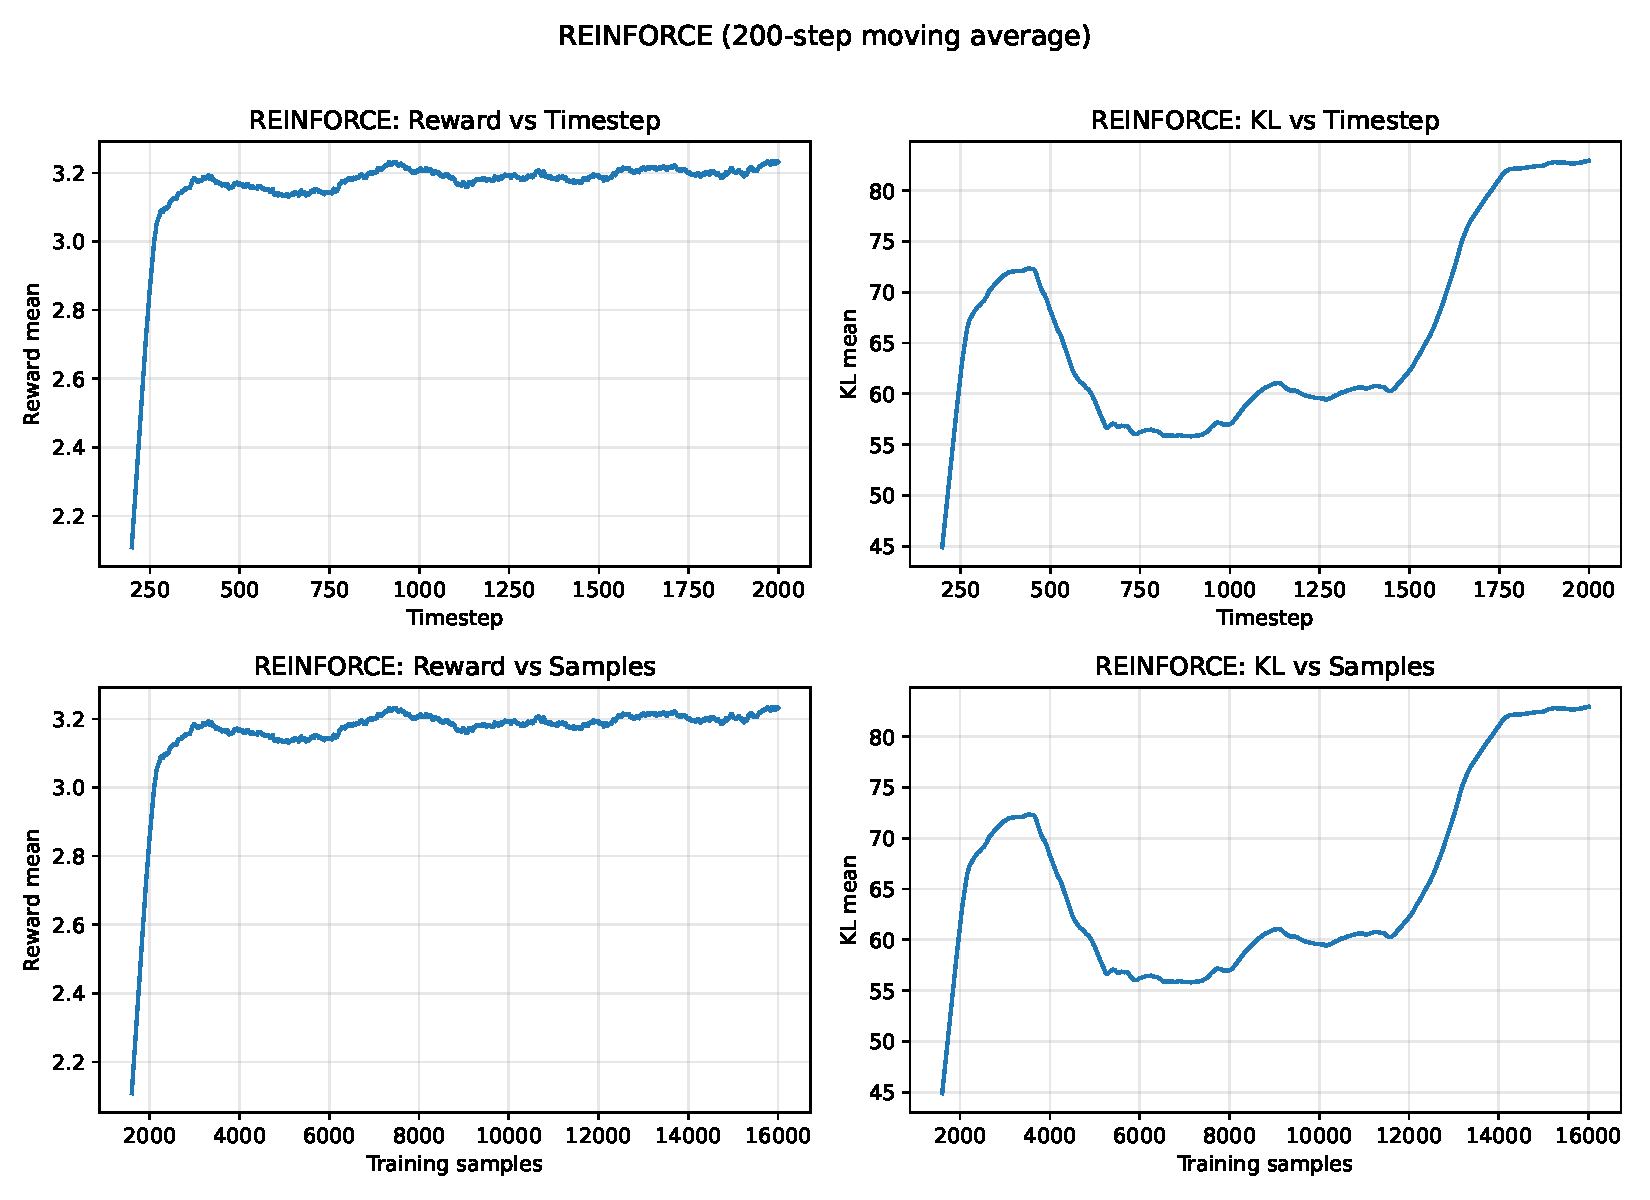
\includegraphics[width=0.9\textwidth]{figures/reinforce.pdf}
\caption{REINFORCE: noisy reward improvement and steadily growing KL, reflecting
the high variance of the raw policy gradient.}
\label{fig:reinforce}
\end{figure}

\subsection{Explicit KL-Regularised REINFORCE}
Increasing the KL weight changes REINFORCE substantially
(Figure~\ref{fig:explicitkl}). The KL is actively controlled and settles at a lower
level than the unregularised baseline (about 56 against 84 in these runs), the
reward plateaus earlier and at a slightly lower value, and training becomes more
stable. This makes the underlying trade-off explicit: optimisation now balances
reward against proximity to the biological prior.

\begin{figure}[h]
\centering
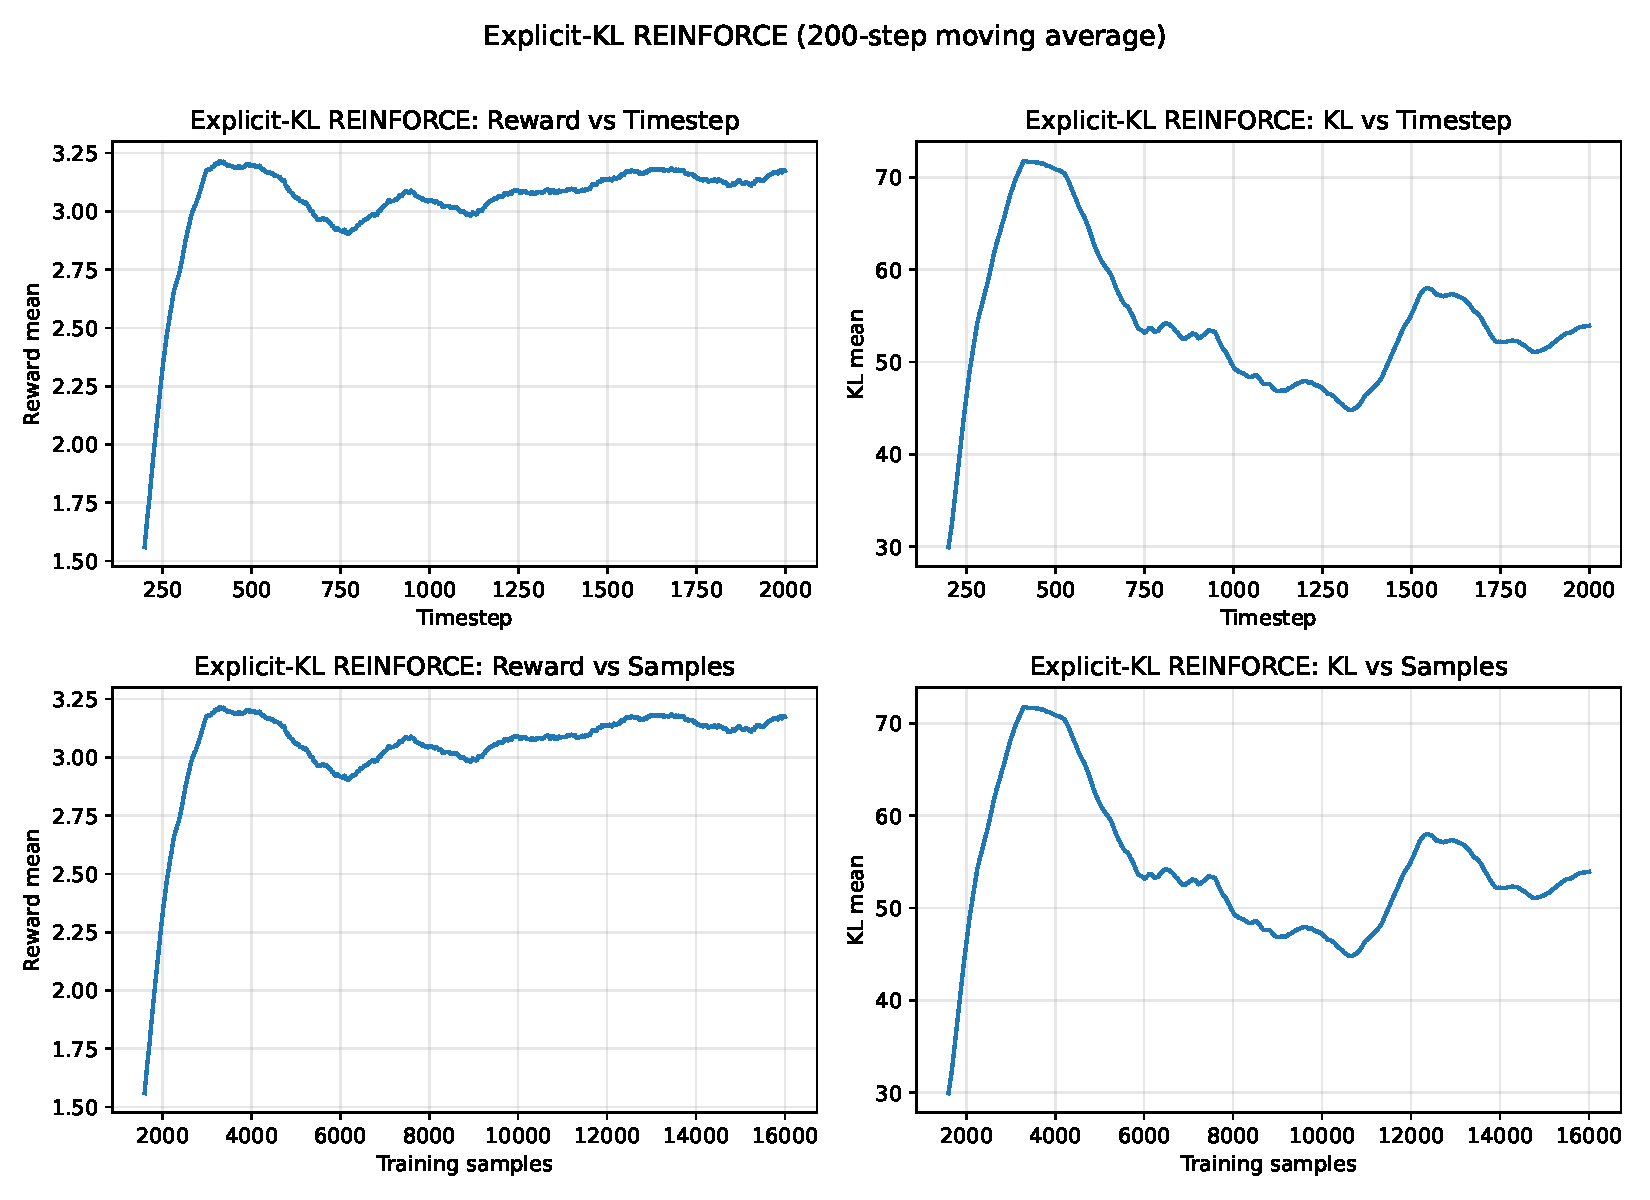
\includegraphics[width=0.9\textwidth]{figures/explicit_kl.pdf}
\caption{Explicit-KL REINFORCE: a stronger KL penalty holds the divergence lower
and stabilises training, at the cost of a slightly lower reward plateau.}
\label{fig:explicitkl}
\end{figure}

\subsection{Convergence and Step Budgets}
Across the online algorithms, most of the reward improvement occurs within roughly
the first one to two thousand steps. Beyond that point the reward gains saturate and
the KL dynamics increasingly dominate, so further training mostly trades biological
realism for marginal proxy improvement. For this task and this proxy, early
optimisation captures most of the useful signal.

\section{Conclusion}
ProteinTuneRL treats antibody design as constrained exploration in sequence space.
This report contributes a precise token-level A2C+GAE formulation for
variable-length infills, together with a correctness pass that makes the KL
regulariser, the value baseline, and the credit-assignment machinery behave as
specified. Several previously silent biases and one gradient-computation failure
are now covered by tests. The reward analysis shows that a tractable proxy must be
interpreted with care, because optimising a compositional statistic does not
guarantee an improvement in the folded structure. Across PPO, A2C, and REINFORCE
the algorithms differ mainly in how far they drift from the pretrained
distribution, which supports the view that the central difficulty here is
controlling divergence from the biological prior while making measurable progress
on the design objective.

\section{Future Work}
Several directions follow from this study. A more faithful reward would score
predicted structure rather than amino-acid composition; folding-based confidence is
already available in the framework but is far more expensive per step, so efficient
approximations are worth exploring. The region-only reward should be recalibrated so
that its normalisation matches the infilled-span distribution. Multi-objective and
constrained formulations would let developability and binding proxies be optimised
jointly rather than through a single scalar. Critic-free, group-relative estimators
offer a lighter alternative to the token-level critic for very short episodes.
Finally, the proxy objectives should be validated against measured biological
properties on a held-out set, so that proxy improvement can be linked to real
design quality.

\section*{Acknowledgements}
This project builds on the ProteinTuneRL framework and on \iglm{} as the underlying
antibody language model. The algorithmic extensions, correctness analysis, and
experiments reported here were carried out on top of that codebase.

\begin{thebibliography}{9}
\bibitem{iglm} R.~Shuai, J.~Ruffolo, J.~Gray. \emph{Generative language modeling
for antibody design.} Cell Systems, 2023.
\bibitem{ppo} J.~Schulman, F.~Wolski, P.~Dhariwal, A.~Radford, O.~Klimov.
\emph{Proximal Policy Optimization Algorithms.} arXiv:1707.06347, 2017.
\bibitem{gae} J.~Schulman, P.~Moritz, S.~Levine, M.~Jordan, P.~Abbeel.
\emph{High-Dimensional Continuous Control Using Generalized Advantage
Estimation.} arXiv:1506.02438, 2015.
\bibitem{ziegler} D.~M.~Ziegler et al. \emph{Fine-Tuning Language Models from Human
Preferences.} arXiv:1909.08593, 2019.
\end{thebibliography}

\end{document}
